\documentclass{beamer}
\usepackage{babel}
\usepackage[utf8]{inputenc}
\usepackage[T1]{fontenc}
\usepackage{graphicx}
\usepackage{stmaryrd}
\usepackage{xcolor}
\usepackage{tikz}
\usepackage{proof}
\usepackage{bussproofs}
\usepackage{listings}
\usepackage{amsmath}

\usetheme{Copenhagen}
\usefonttheme{professionalfonts}
\setbeamertemplate{navigation symbols}{}
\setbeamertemplate{headline}{}

\definecolor{delimiterColor}{HTML}{B65E47}
\definecolor{numberColor}{HTML}{FF0000}
\definecolor{commentColor}{HTML}{008000}
\definecolor{keyColor}{HTML}{002BFF}

\lstdefinelanguage{maude}
{
	breaklines=true,
	extendedchars=true,
	tabsize=2,
	frame=none,
	columns=fullflexible,
	showtabs=false,
	showstringspaces=false,
	showspaces=false,
	showstringspaces=false,
	identifierstyle={\ttfamily},
	keywordstyle={\color{keyColor}},
	ndkeywordstyle={\color{keyColor}},
	stringstyle={\color{delimiterColor}},
	commentstyle={\color{commentColor}},
	ndkeywords={Int, Bool, String},
	keywords={in, load, pr, protecting, sort, sorts, op, ops, var, vars,eq, cq, ceq,endfm, fmod, is, mod, endm, load, =, ==, =/=, euler, discreteswitch, nonaccurate, mp, rk4, accurate, init, exp, abs, true, false, nil, ctor, PhysicalEntityStar, PhysicalInteraction, PhysicalEntity, PhysicalEntityPC1, FlowSource, SysMan, effortDyn, flowDyn, Object, Oid, assoc, comm, id, DataCollector, Rat, NzNat, frac, trunc, if, else, class, load, homod, endhom, eof, var, vars, eq, op, ops, pr, inc, protecting, including, ceq, is, tomod, endtom, msg, rl, crl, trew, hfind, hsearch, tsearch, hmc, hrew, time, earliest, such, that, subclass, Prop, omod, sort, subsort, not, endom, fi, msgs, fmod, endfm, hfrew, then, mod, and, or, endm, endtm, in, out, set, trace, exclude, loop, show, using, stepsize, tick, Oid, Nat, Float, Configuration, String, NzNat},
	morecomment={[l]{***}},
	morecomment={[l]{---}},
}
\AtBeginSection[ ]
{
\begin{frame}{Outline}
    \tableofcontents[currentsection, hideallsubsections]
\end{frame}
}
\title{Conditional Rewriting Logic \& Maude}
\author{Niccolò Piazzesi}
\institute{
    Università degli studi di Pisa
}
\titlegraphic{
\includegraphics[width=2cm]{img/logo.png}}
\begin{document}

\frame{\titlepage}

\begin{frame}{Outline}
    \tableofcontents[hideallsubsections]
\end{frame}
\section{Introduction and main concepts}
\begin{frame}
    \frametitle{What is a concurrent system?}
    Modelling concurrent system is one of the most studied problems in Computer Science.

    \bigskip
    \pause
    Many proposed answers:\begin{itemize}
        \item Petri Nets 
        \item CCS
        \item CSP 
        \item Actors
        \item $\cdots$
    \end{itemize}
\end{frame}
\begin{frame}
    \frametitle{The need for unification}
    \pause
        \begin{block}{External fragmentation}
            Hard to relate different approaches, each with their own concepts, models and issues.
        \end{block}
    \pause 
    \begin{block}{Internal fragmentation}
        Sometimes, fragmentation appears also within a specific approach (e.g. how can we unify operational and denotational semantics of CCS?).
    \end{block}
    \pause
    \begin{block}{Concurrency in other areas}
        A related problem is the integration of concurrency with other paradigms ( OO, Functional, ...)
        without using complex \emph{ad hoc} solutions.
    \end{block}
\end{frame}

\begin{frame}
    
    Rewriting logic aim to resolve these issues with a two sides approach.
    \pause
    \begin{block}{Computational side}
        Computationally, rewriting logic is a \emph{semantic framework} where many different 
        models and languages can be represented and executed as \textbf{rewrite theories}. 
    \end{block}
    \pause
    \begin{block}{Logical side}
        Rewriting logic  is also a \emph{logical framework}, a model within which 
        many other logics and deduction procedures  can be modeled and reasoned about.        
    \end{block}
\end{frame}
\section{Foundations}
\begin{frame}
    \frametitle{A logic of action}
    The rules of rewriting logic resemble those of equational logic, but the meaning is very different.

    \begin{center}
        \textbf{Rewriting logic is a logic to reason about \emph{change} in a concurrent system, \emph{not about equality.}}
    \end{center}
\pause 

\bigskip 
Rewriting logic identifies \textbf{concurrent rewriting} with \textbf{deduction}.
\end{frame}

\begin{frame}
    \frametitle{Rewrite Theory}
    \begin{center}
        \resizebox{3cm}{!}{$(\Sigma, E, L, R)$}
    \end{center}
    
    \bigskip
    \begin{itemize}
        \pause
        \item $\Sigma$: ranked alphabet of function symbols
        \pause
        \item E: set  of $\Sigma$-equations 
        \pause
        \item L: set of \emph{labels}
        \pause
        \item R: set of pairs $R \subseteq L \times (T_{\Sigma, E}(\mathbf{X})^2)^+$
    \end{itemize}
    
    \pause
    \bigskip
    $T_{\Sigma,E}(\mathbf{X})$ denotes the $\Sigma-algebra$ of equivalence classes of $\Sigma-terms$ with variables in $\mathbf{X}$ modulo the equations E.
    
    \medskip
    Elements of R are called \emph{rewrite rules}.
\end{frame}
\begin{frame}
    \frametitle{Rewriting rules}
    A rewrite rule 
    \begin{center}
        $(r,([t],[t'])([u_1],[v_1])\cdots([u_k],[v_k]))$
    \end{center}
    is written as 
    $$
    r:[t] \rightarrow [t']\ if\ \underbrace{[u_1]\rightarrow[v_1] \wedge \cdots \wedge [u_k] \rightarrow [v_k] \pause}_{condition\ C}
    $$
    
    \bigskip
    \pause
    If a condition is empty, we have an \emph{unconditional rewrite rule}.
    $$
    r:[t] \rightarrow [t']
    $$
    

    If all the rules are unconditional , we have an \emph{unconditional rewrite theory}
\end{frame}
\begin{frame}

    An example: natural numbers with a nondeterministic choice operator 
    
    \pause
    \begin{itemize}
        \item $\Sigma = \{0,s\_,\_+\_,\_?\_\}$
        \pause
        \item $E = \{N + M = M + N\}$
        \pause
        \item R = 
            \vspace{-5mm}
            \begin{align*}
                &r1: N+0 \rightarrow N \\ 
                &r2: (s\ N) + (s\ M) \rightarrow s\ s\ (N + M) \\ 
                &r3: N ? M \rightarrow N \\ 
                &r4: N ? M \rightarrow M 
            \end{align*}
    \end{itemize}
\end{frame}
\begin{frame}
    \frametitle{Sequent entailment}
    \begin{center}
        \resizebox{3cm}{!}{$\mathcal{R} \vdash [t] \rightarrow [t']$}
    \end{center}

    \pause 
    \vspace{2cm}
    A rewrite theory $\mathcal{R}$ \emph{entails} a \emph{sequent}
    $ [t] \rightarrow [t']$ \emph{iff} $[t] \rightarrow [t']$ can be obtained 
    by finite application of \emph{rules of deduction}.
\end{frame}
\begin{frame}[allowframebreaks]
    \frametitle{Rules of deduction}
    \scriptsize
    \begin{enumerate}
        \item \emph{Relfexivity}. For each $[t] \in T_{\Sigma,E}(\mathbf{X})$, 
            $$
            \infer[]{[t] \rightarrow [t']}{}
            $$
        \item \emph{Congruence}. For each $f \in \Sigma_n, n \in \mathbb{N}$,
            $$
            \infer[]{[f(t_1,\cdots,t_n)] \rightarrow [f(t_1',\cdots,t_n')]}{[t_1] \rightarrow [t_1']\ \cdots\ [t_n] \rightarrow [t_n']}            $$ 
        \item \emph{Replacement}. For each rule  
        \begin{align*}
            r&:[t(\overline{x})] \rightarrow [t'(\overline{x})]\ if \\
            &[u_1(\overline{x})] \rightarrow [v_1(\overline{x})] \wedge \cdots \wedge [u_n(\overline{x})] \rightarrow [v_n(\overline{x})]
        \end{align*}
        in $R$,
        \begin{prooftree}
            \alwaysNoLine
            \AxiomC{$[w_1] \rightarrow [w_1']$}
            \UnaryInfC{$[u_1(\overline{w}/ \overline{x})] \rightarrow [v_1(\overline{w}/ \overline{x})]$}
                \AxiomC{$\cdots$}
                \UnaryInfC{$\cdots$}
                    \AxiomC{$[w_n] \rightarrow [w_n']$}
                    \UnaryInfC{$[u_k(\overline{w}/ \overline{x})] \rightarrow [v_k(\overline{w}/ \overline{x})]$}
                \alwaysSingleLine
                \TrinaryInfC{$[t(\overline{w}/ \overline{x})] \rightarrow [t'(\overline{w}'/ \overline{x})]$}
        \end{prooftree}

        \item \emph{Transitivity}
        $$
        \infer[]{[t_1] \rightarrow [t_3]}{[t_1] \rightarrow [t_2] \quad [t_2] \rightarrow [t_3]} 
        $$
        \item \emph{Unconditional replacement}. For each 
        $$ r: [t(x_1,\cdots,x_n)] \rightarrow [t'(x_1,\cdots,x_n)]$$
        in R, 
        $$
        \infer[]{[t(\overline{w} / \overline{x} )] \rightarrow [t'(\overline{w'} / \overline{x})]}{[w_1] \rightarrow [w_1'] \quad \cdots \quad [w_n] \rightarrow [w_n']}
        $$
    \end{enumerate}
\end{frame}
\begin{frame}
    \frametitle{Additional rules}
    \scriptsize
    \begin{enumerate}
        \setcounter{enumi}{5}
        \item \emph{Substitution}
        $$
        \infer[]
        {[t(w_1)/x_{i_1},\cdots,w_n/x_{i_n}] \rightarrow [t'(w_1')/x_{i_1},\cdots,w_n'/x_{i_n}]}
        {[t(x_{i_1},\cdots,x_{i_n})] \rightarrow [t'(x_{i_1},\cdots,x_{i_n})] \quad [w_1] \rightarrow [w_1'] \cdots [w_n] \rightarrow [w_n']} 
        $$
    \end{enumerate}
    
    Any sequent derivable by adding (6) to  (1)-(4) can be derived by using only (1)-(4).

    \pause 
    \bigskip
    \emph{Equational logic} can be obtained  from rewriting logic by adding the following rule:
    \begin{enumerate}
        \setcounter{enumi}{6}
        \item \emph{Simmetry}
        $$
        \infer[]{[t_2] \rightarrow [t_1]}{[t_1] \rightarrow [t_2]} 
        $$
    \end{enumerate}
    \pause 
    
    \bigskip 
    We can now give the definition of \emph{concurrent rewriting}.
\end{frame}
\begin{frame}
    \frametitle{Concurrent rewriting}
    $\mathcal{R} = (\Sigma, E, L, R)$
    \small
    
    \pause
    \medskip
    A $(\Sigma, E)$ sequent $[t] \rightarrow [t']$ is called:\begin{itemize}
        \item a \emph{0-step concurrent $\mathcal{R}$-rewrite} iff it can be derived from $\mathcal{R}$ by finite application 
        of rules (1) and (2).
        \pause
        \item a \emph{one-step concurrent $\mathcal{R}$-rewrite} iff it can be derived from $\mathcal{R}$
        by finite applications of rules (1)-(3), with at least one application of (3).
        \pause
        \item a \emph{concurrent $\mathcal{R}$-rewrite} iff it can be derived from $\mathcal{R}$ by finite applications of rules (1)-(4).
    \end{itemize}
\end{frame}
\begin{frame}
    $\mathcal{R} = (\Sigma, E, L, R)$
    \small
    \begin{block}{Lemma}
        For each concurrent $\mathcal{R}$-rewrite $[t] \rightarrow [t']$
        either $[t] = [t']$ or there is a $n  \in \mathbb{N} $ and a chain  of one step (concurrent) rewrites 
        $$
        \underbrace{[t] \rightarrow [t_1] \rightarrow \cdots \rightarrow [t_n] \rightarrow [t'] \onslide<2->}_{step\ seqeunce}
        $$ 
    \end{block}

    \onslide<3->{
    \medskip
    $\mathcal{R}$ is \emph{terminating} if there is no infinite chain of one step rewrites.

    \medskip
    $[t']$ is an $\mathcal{R}-normal\ form$ of $[t]$ if $[t] \rightarrow [t']$ is an 
    $\mathcal{R}$-rewrite and there is no $[t'] \rightarrow [t'']$ one-step  $\mathcal{R}$-rewrite.
    }

    \onslide<4->{
    
    \medskip
    $\mathcal{R}$ is \emph{Church-Rosser} or \emph{confluent} if
    \begin{figure}
        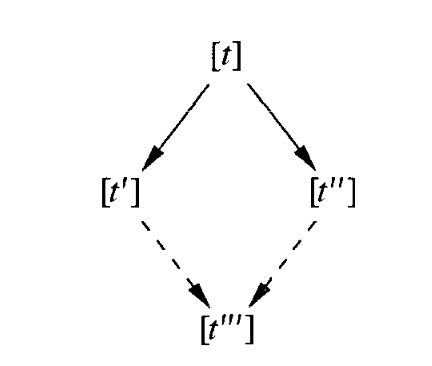
\includegraphics[scale=0.2]{img/churchrosser.png}
    \end{figure}
    }
\end{frame}
\begin{frame}
    \frametitle{Reflection}

    Rewriting logic is \textbf{reflective}.

    \pause 
    \bigskip 
    There is a finitely presented rewrite theory $\mathbf{U}$ such that, for 
        any finitely presented rewrite theory $\mathbf{T}$ (including $\mathbf{U}$ itself) we have 
        the following equivalence:
        $$
        T \vdash [t] \rightarrow [t'] \Longleftrightarrow U \vdash  \langle \overline{T},\overline{[t]} \rangle  \rightarrow \langle \overline{T},\overline{[t']} \rangle
        $$ 

    \pause 
    This property is fundamental for the applications of RL, as we will see in Maude.
\end{frame}
\section{Semantic model}
\begin{frame}
    \begin{block}{What we have}
    $ R = (\Sigma, E, L, R)$

    \emph{Static description} of what a system can do.
        
    \end{block}
    
    \pause

    \begin{block}{What we want}
        \emph{Computational models} of the system behaviour (the \emph{meaning of the theory}).
    \end{block}

    \pause

    \begin{block}{Idea}
        Take advantage of the correspondence between  \emph{deductions} in rewriting logic 
        and \emph{concurrent computations}.
    \end{block}
\end{frame}
\begin{frame}
    \frametitle{The model }
    $
    R = (\Sigma, E, L, R)
    $

    \pause 
    \bigskip
    We seek a \textcolor{red}{category} $\mathcal{T_R(X)}$:\begin{itemize}
        \item Objects: \textcolor{blue}{$[t]_E$}
        \item Arrows: \textcolor{blue}{$[t_1]_E \xrightarrow{\pi} [t_2]_E$}
    \end{itemize}

    \pause 
    \bigskip
    \emph{Generator rules}: obtained by the rules of deduction (1)-(4) by decorating 
    the sequents with appropriate proof terms.
\end{frame}
\begin{frame}
    \frametitle{Rules of generation}
    \scriptsize 
    \begin{enumerate}
        \item \emph{Identities.} For each $[t] \in T_{\Sigma, E}(\mathbb{X})$,
        $$
        \infer[]{[t]: [t] \rightarrow [t]}{}
        $$

        \item $\Sigma-structure$. For each $f \in \Sigma_n, n \in \mathbb{N}$,
        $$
        \infer[]
        {f(\alpha_1, \cdots, \alpha_n): [f(t_1, \cdots, t_n)] \rightarrow [f(t_1', \cdots, t_n')]}
        {\alpha_1: [t_1]}
        $$

        \item \emph{Replacement.} For each rewrite rule 
        \begin{align*}
        r:&[t(\overline{x})] \rightarrow [t'(\overline{x})]\ if \\ 
        &[u_1(\overline{x})] \rightarrow [v_1(\overline{x})] \wedge \cdots \wedge [u_k(\overline{x})] \rightarrow [v_k(\overline{x})] 
        \end{align*}
        in $\mathbb{R}$,
        \begin{prooftree}
            \alwaysNoLine
            \AxiomC{$\alpha_1 : [w_1] \rightarrow [w_1']$}
            \UnaryInfC{$\beta_1 : [u_1(\overline{w}/ \overline{x})] \rightarrow [v_1(\overline{w}/ \overline{x})]$}
                \AxiomC{$\cdots$}
                \UnaryInfC{$\cdots$}
                    \AxiomC{$\alpha_n : [w_n] \rightarrow [w_n']$}
                    \UnaryInfC{$\beta_k : [u_k(\overline{w}/ \overline{x})] \rightarrow [v_k(\overline{w}/ \overline{x})]$}
                \alwaysSingleLine
                \TrinaryInfC{$r(\overline{\alpha}^n,\overline{\beta}^k)[t(\overline{w}/ \overline{x})] \rightarrow [t'(\overline{w}'/ \overline{x})]$}
        \end{prooftree}

        \item \emph{Composition}
        $$
        \infer[]{\alpha;\beta : [t_1] \rightarrow [t_3]}{\alpha : [t_1] \rightarrow [t_2] \quad \beta : [t_2] \rightarrow [t_3]} 
        $$
    \end{enumerate}
\end{frame}
\begin{frame}
    For equational logic we can define a similar category $\mathcal{T_R}^{\leftrightarrow}(X)$ ( a \emph{groupoid}) by using 
    the rule of simmetry to generate additional terms:
    
    \bigskip 
    {
    \scriptsize
    \begin{enumerate}
        \setcounter{enumi}{4}
        \item  \emph{Inversion}. 
        $$
        \infer[]{\alpha^{-1} : [t_2] \rightarrow [t_1]}{\alpha : [t_1] \rightarrow [t_2]}
        $$
    \end{enumerate}
    }

    \bigskip
    \pause 
    \textbf{Note:}

    Ambiguity problems, which may arise when  the same label \emph{r} appears in two different rules of R, are assumed 
    to be resolved by disambiguating \emph{r}  in the proof term $r(\overline{\alpha},\overline{\beta})$.
\end{frame}
\begin{frame}
    \frametitle{$\mathcal{P_R}(X)$}

    Each of the generation rules (1)-(4) defines an operation taking certain proof terms as argument and returning 
    a resulting proof term.

    \bigskip
    \pause 
    In other words, proof terms form an algebraic structure $\mathcal{P_R}(X)$ defined by the generation rules.

    \bigskip
    \pause 
    More specifically, the generated structure is a graph $\mathcal{G}$ where: 
    \begin{itemize}
        \item $Nodes = T_{\Sigma,E}(X)$
        \item $Arrows = \mathcal{P_R}(X)$
        \item $\partial_0 (\textbf{source}), \partial_1 (\textbf{target}) : \mathcal{P_R}(X) \rightarrow T_{\Sigma,E}(X)$
    \end{itemize}
\end{frame}
\begin{frame}
    \scriptsize
    Rule (1) requires each node $[t]$ to also be an arrow $[t] : [t] \rightarrow [t]$, making $\mathcal{G}$ \emph{reflexive}.

    \bigskip
    \pause

    By rule (2), $\mathcal{P_R}(X)$ has a $\Sigma$-algebra structure where $\partial_0,\partial_1$ are 
    $\Sigma$-omomorphisms.

    \bigskip
    \pause
    Rule (4) defines a new operation:
    $$
    \_;\_ : Composable(\mathcal{P_R(X)}) \rightarrow \mathcal{P_R(X)}
    $$
    where $\partial_0(a;b) = \partial_0(a)$ and $\partial_1(a;b) = \partial_1(b)$.

    \bigskip
    \pause
    By rule (3),for each rewrite rule 
    \begin{align*}
        r:&[t(\overline{x})] \rightarrow [t'(\overline{x})]\ if \\ 
        &[u_1(\overline{x})] \rightarrow [v_1(\overline{x})] \wedge \cdots \wedge [u_k(\overline{x})] \rightarrow [v_k(\overline{x})] 
    \end{align*}
    we define an operation 
    \begin{align*}
        r(\_,_) : \{(\overline{\alpha}^n,\overline{\beta}^k) \in \mathcal{P_R}(X&)^{n+k} 
        | \partial_0^k(\overline{\beta}^k) = \overline{[u(\partial_0^n(\overline{\alpha}^n)\overline{x})]}^k \\
        &\wedge  \partial_1^k(\overline{\beta}^k) = \overline{[v(\partial_0^n(\overline{\alpha}^n)\overline{x})]}^k\} \rightarrow \mathcal{P_R}(X)
    \end{align*}
\end{frame}
\begin{frame}
    \scriptsize
    \begin{block}{R-presystem}
        Given a rewrite theory $\mathcal{R} = (\Sigma, E, L, R)$, an $\mathcal{R}-presystem$
        is a reflexive graph $G$ together with: \begin{enumerate}
            \item a $\Sigma$-algebra structure onn $G$ such that the $\Sigma$-algebra Nodes of nodes
            satisfies the equation in $E$;
            \item an operation 
            $$ \_;\_ : Composable(G) \rightarrow Arrows$$
            with $\partial_0(a;b) = \partial_0(a)$ and $\partial_1(a;b) = \partial_1(b)$
            \item for each rewrite rule 
            \begin{align*}
                r:&[t(\overline{x})] \rightarrow [t'(\overline{x})]\ if \\ 
                &[u_1(\overline{x})] \rightarrow [v_1(\overline{x})] \wedge \cdots \wedge [u_k(\overline{x})] \rightarrow [v_k(\overline{x})] 
            \end{align*}
            in $R$, an operation  
            \begin{align*}
                r(\_,_) : \{(\overline{a}^n,\overline{b}^k) \in Arrows^{n+k}& 
                | \partial_0^k(\overline{b}^k) = \overline{u_{Nodes}(\partial_0^n(\overline{a}^n))}^k \\
                &\wedge  \partial_1^k(\overline{b}^k) = \overline{v_{Nodes}(\partial_0^n(\overline{a}^n))}^k\} \rightarrow Arrows
            \end{align*}
        such that $$ r(\overline{a}^n,\overline{b}^k) : t_{Nodes}(\partial_0^n(\overline{a}^n)) \rightarrow t_{Nodes}'(\partial_1^n(\overline{a}^n))$$
        \end{enumerate}
    \end{block}
\end{frame}
\begin{frame}
    \small
    \begin{block}{$\mathcal{R}$-prehomomorphism}
        Given two $\mathcal{R}$-presystems G and G', an $\mathcal{R}$-prehomomorphism is a 
        graph omomorphism that preserves all the operations in $\Sigma$, the operation $\_;\_$ and the operation $r(\_,\_)$ for $r \in R$.
        With this, we can define the category $\underline{\mathcal{R}\text{-PreSys}}$.
    \end{block}
    
    \pause
    \begin{block}{Propostion}
        The forgetful functor 
        $$Nodes: \underline{\mathcal{R}\text{-PreSys}} \rightarrow \underline{Set}$$
        sending each $\mathcal{R}$-presystem to its set of nodes has a left adjoint.
    \end{block}
\end{frame}

\begin{frame}[allowframebreaks]
    \scriptsize
    \frametitle{$\mathcal{T_R}(X)$}
    Given a rewrite theory $\mathcal{R}$, the model $\mathcal{T_R}(X)$ is the quotient of 
    $\mathcal{P_R}(X)$ modulo the following equations:
    
    \begin{enumerate}
        \item \emph{Category}.
        \begin{enumerate}[a]
            \scriptsize
            \item Associativity. For all $\alpha,\beta,\gamma$,
            
            $(\alpha;\beta);\gamma = \alpha;(\beta;\gamma).$
            \item Identities. For each $\alpha: [t] \rightarrow [t']$,
            
            $\alpha;[t'] = \alpha,\quad [t];\alpha=\alpha.$
        \end{enumerate}
        \item \emph{Functioriality.}. For each $f \in \Sigma_n, n \in \mathbb{N}$,
        \begin{enumerate}[a]
            \scriptsize
            \item Preservation of composition. For all $\alpha_1,\cdots,\alpha_n,\beta_1,\cdots,\beta_n$,
            
            $f(\alpha_1;\beta_1,\cdots,\alpha_n;\beta_n) = f(\alpha_1,\cdots,\alpha_n);f(\beta_1,\cdots,\beta_n). $
            \item Preservation of Identities.
            
            $ f([t_1],\cdots,[t_n])=[f(t_1,\cdots,t_n)].$
        \end{enumerate}
        \item \emph{Axioms} in $E$. For $t(x_1,\cdots,x_n)=t'(x_1,x_n)$ an axiom in $E$, for all $\alpha_1,\cdots,\alpha_n$,
        
        $ t(\alpha_1,\cdots,\alpha_n)=t'(\alpha_1,\cdots,\alpha_n).$

        \item \emph{Decomposition}.  For each rewrite rule 
        \begin{align*}
        r:&[t(\overline{x})] \rightarrow [t'(\overline{x})]\ if \\ 
        &[u_1(\overline{x})] \rightarrow [v_1(\overline{x})] \wedge \cdots \wedge [u_k(\overline{x})] \rightarrow [v_k(\overline{x})] 
        \end{align*}
        in $\mathbb{R}$,
        \begin{prooftree}
            \alwaysNoLine
            \AxiomC{$\alpha_1 : [w_1] \rightarrow [w_1']$}
            \UnaryInfC{$\beta_1 : [u_1(\overline{w}/ \overline{x})] \rightarrow [v_1(\overline{w}/ \overline{x})]$}
                \AxiomC{$\cdots$}
                \UnaryInfC{$\cdots$}
                    \AxiomC{$\alpha_n : [w_n] \rightarrow [w_n']$}
                    \UnaryInfC{$\beta_k : [u_k(\overline{w}/ \overline{x})] \rightarrow [v_k(\overline{w}/ \overline{x})]$}
                \alwaysSingleLine
                \TrinaryInfC{$r(\overline{\alpha}^n,\overline{\beta}^k) = r([\overline{w}]^n,\overline{\beta}^k);t'(\overline{\alpha}^n)$}
        \end{prooftree}
        \item \emph{Exchange}. For each rewrite rule 
        \begin{align*}
        r:&[t(\overline{x})] \rightarrow [t'(\overline{x})]\ if \\ 
        &[u_1(\overline{x})] \rightarrow [v_1(\overline{x})] \wedge \cdots \wedge [u_k(\overline{x})] \rightarrow [v_k(\overline{x})] 
        \end{align*}
        in $\mathbb{R}$,
        \begin{prooftree}
            \alwaysNoLine
            \AxiomC{$\alpha_1 : [w_1] \rightarrow [w_1']$}
            \UnaryInfC{$\beta_1 : [u_1(\overline{w}/ \overline{x})] \rightarrow [v_1(\overline{w}/ \overline{x})]$}
            \UnaryInfC{$\beta_1' : [u_1(\overline{w'}/ \overline{x})] \rightarrow [v_1(\overline{w'}/ \overline{x})]$}
            \UnaryInfC{$\beta_1;v_1(\overline{\alpha}) = u_1(\overline{\alpha});\beta_1'$}
                \AxiomC{$\cdots$}
                \UnaryInfC{$\cdots$}
                \UnaryInfC{$\cdots$}
                \UnaryInfC{$\cdots$}
                \UnaryInfC{$\cdots$}
                    \AxiomC{$\alpha_n : [w_n] \rightarrow [w_n']$}
                    \UnaryInfC{$\beta_k : [u_k(\overline{w}/ \overline{x})] \rightarrow [v_k(\overline{w}/ \overline{x})]$}
                    \UnaryInfC{$\beta_k' : [u_k(\overline{w'}/ \overline{x})] \rightarrow [v_k(\overline{w'}/ \overline{x})]$}
                    \UnaryInfC{$\beta_k;v_k(\overline{\alpha}) = u_k(\overline{\alpha});\beta_k'$}
                \alwaysSingleLine
                \TrinaryInfC{$r(\overline{[w]}^n,\overline{\beta}^k);t'(\overline{\alpha}) = t(\overline{\alpha});r([\overline{w'}]^n,\overline{\beta'}^k)$}
        \end{prooftree}
    \end{enumerate}
    
\end{frame}
\begin{frame}
    
    The groupoid $\mathcal{T_R}^{\leftrightarrow}(X)$ is obtained by adding the rule:
    \begin{enumerate}
        \setcounter{enumi}{5}
        \item  \emph{Inverse.} For any $\alpha:[t] \rightarrow [t']$ in $\mathcal{T_R}^{\leftrightarrow}(X)$, 
    
        $ \alpha;\alpha^{-1} = [t],\quad \alpha^{-1};\alpha= [t'].$
    \end{enumerate}
    \pause
    \begin{block}{Lemma}
        For each $ r:[t(x_1,\cdots,x_n)] \rightarrow [t'(x_1,\cdots,x_n)]$ in $R$, the \emph{family of morphisms}
        $$ \{r(\overline{[w]}): [t(\overline{w}/\overline{x})] \rightarrow [t'(\overline{w}/\overline{x})] | \overline{[w]} \in T_{\Sigma,E}(X)^n\}$$
        is a natural transformation
        $$ r:[t(x_1,\cdots,x_n)] \Rightarrow [t'(x_1,\cdots,x_n)]$$
        between the functors 
        $$[t(x_1,\cdots,x_n)],[t'(x_1,\cdots,x_n)]: \mathcal{T_R}(X)^n \rightarrow \mathcal{T_R}(X).$$

    \end{block}
\end{frame}
\begin{frame}
    We can now make precise the mathematical meaning of the \emph{exchange} law.
    
    \pause 
    \begin{block}{Subequalizer}
        Given functors F,G:$\mathcal{A} \rightarrow \mathcal{B}$, the \textbf{\emph{subequalizer}} of F and G is a 
        category $Subeq(F,G)$ together with a functor $J:Subeq(F,G) \rightarrow \mathcal{A}$ and a natural transformation 
        $\alpha: J *  F \Rightarrow J * G$ satisfying the following universal property:

        \bigskip
        Given a functor $H:\mathcal{C} \rightarrow \mathcal{A}$ and  a natural transformation $\beta:H*F \Rightarrow H*G$, there exists a unique functor 
        $ (H,\beta):\mathcal{C} \rightarrow Subeq(F,G)$ such that 
        $$ (H,\beta) * J = H\ and\ (H,\beta)*\alpha = \beta.$$ 

        For a family of pair of functors $\{F_i,G_i:\mathcal{A} \rightarrow \mathcal{B}_i | i \in I\}$,
        $$ (H,\{\beta_i\}_{i \in I}) * J = H\ and\ (H,\{\beta_i\}_{i \in I})*\alpha_i = \beta_i (i \in I).$$ 
    \end{block}
    

\end{frame}
\begin{frame}
    \scriptsize
    $\mathbf{Subeq((F_i,G_i)_{i \in I})}$:
    \begin{itemize}
        \item Objects : $(A,\{b_i\}_{i \in I})$ where $A$ object in $\mathcal{A}$ and $b_i:F_i(A) \rightarrow G_i(A)$ a morphism in $\mathcal{B}_i$.
        \item Arrows : $$ a: (A,\{b_i\}_{i \in I}) \rightarrow (A',\{b_i\}_{i \in I})$$
        are morphisms $a: A \rightarrow A'$ in $\mathcal{A}$ such that for each $i \in I,b_i;G_i(A)=F_i(a);b_i'.$
    \end{itemize}

    \bigskip
    \pause 
    Functor J is the projection into the first component. The natural transformation $\alpha_j$ is defined by 
    $$\alpha_j(A,\{b_i\}_{i \in I}) =  b_j.$$ 

    \bigskip
    \pause
    For the exchange law, we are interested in subequalizers of the form 
    $$ Subeq(([u_j(\overline{x})],[v_j(\overline{x})])_{1 \le j \le k}) $$ 
    associated  to rewrite rules 
    \begin{align*}
        r:&[t(\overline{x})] \rightarrow [t'(\overline{x})]\ if \\ 
        &[u_1(\overline{x})] \rightarrow [v_1(\overline{x})] \wedge \cdots \wedge [u_k(\overline{x})] \rightarrow [v_k(\overline{x})] 
    \end{align*} 
\end{frame}
\begin{frame}
    \begin{block}{Lemma}
        For each rewrite rule
        \begin{align*}
            r:&[t(\overline{x})] \rightarrow [t'(\overline{x})]\ if \\ 
            &[u_1(\overline{x})] \rightarrow [v_1(\overline{x})] \wedge \cdots \wedge [u_k(\overline{x})] \rightarrow [v_k(\overline{x})] 
            \end{align*}
        in $R$, the \emph{family of morphisms}
        \begin{align*}
            \{r(\overline{[w]}^n,\overline{\beta}^k):&[t(\overline{w}/ \overline{x})] \rightarrow [t'(\overline{w}/ \overline{x})]\ | \\ 
            &(\overline{[w]}^n,\overline{[\beta]}^k) \in Subeq(([u_j(\overline{x})],[v_j(\overline{x})])_{1 \le j \le k})\}
            \end{align*}
        is a natural transformation 
        $$r: J * [t(x_1,\cdots,x_n)] \Rightarrow J * [t'(x_1,\cdots,x_n)]$$
        where $J: Subeq(([u_j(\overline{x})],[v_j(\overline{x})])_{1 \le j \le k}) \rightarrow \mathcal{T_R}(X)^n$ is the \emph{subequalizer functor}.
    \end{block}
\end{frame}
\begin{frame}
    \scriptsize
    The construction $\mathcal{T_R}$ is very general, includes other constructions as particular cases.

    \pause
   
    $$\mathcal{R} : LTS \Rightarrow  \mathcal{T_R} : \underline{Path}$$

    \pause
    
    $$\mathcal{R} : \text{Petri nets} \Rightarrow  \mathcal{T_R} : \underline{Petri}$$

\pause 
\bigskip
Equations (1)-(5) provides \emph{the most abstract view} of the computations in $\mathcal{R}$. The \emph{decomposition} and \emph{exchange} equations 
tells us that the order of rewrites performed "above" and "below" a term does not matter.
\pause 
\begin{block}{Lemma}
For each $[\alpha]: [t] \rightarrow [t']$ in $\mathcal{T_R}(X)$, either $[t] = [t']$ and 
$[\alpha] = [[t]]$, or there  is an $n \in \mathbb{N}$ and a chain of morphisms $[\alpha_i], 0 \le i \le n$ whose terms 
$\alpha_i$ describe one-step concurrent rewrites 
$$ [t] \xrightarrow{\alpha_0} [t_1] \xrightarrow{\alpha_1} \cdots \xrightarrow{\alpha_{n-1}} [t_n] \xrightarrow{\alpha_n} [t']$$
such that $[\alpha] = [\alpha_0;\cdots;\alpha_n].$

The proof is by induction on the depth of proof terms.
    
\end{block}
\pause 
$\mathcal{T_R}(X)$ is just one among many models for a rewrite theory $\mathcal{R}.$ Let's now see the general model.
\end{frame}
\begin{frame}
    \frametitle{$\mathcal{R}$-systems}
    \scriptsize
    Given a rewrite theory $\mathcal{R} = (\Sigma,E,L,R)$, an \emph{\textbf{$\mathcal{R}$-system $\mathcal{S}$}} is a 
    category $\mathcal{S}$ together with:
    \begin{enumerate}
        \item a $(\Sigma,E)$-algebra structure. For each $f \in \Sigma_n,\ n\in \mathbb{N}$, a functor $f_{\mathcal{S}}:\mathcal{S}^n \rightarrow \mathcal{S}$
        is defined in such a way that 
        $$t(x_1,\cdots,x_n) = t'(x_1,\cdots,x_n) \Rightarrow t_{\mathcal{S}} = t_{\mathcal{S}}'$$
        \item For each rewrite rule
        \begin{align*}
            r:&[t(\overline{x})] \rightarrow [t'(\overline{x})]\ if \\ 
            &[u_1(\overline{x})] \rightarrow [v_1(\overline{x})] \wedge \cdots \wedge [u_k(\overline{x})] \rightarrow [v_k(\overline{x})] 
            \end{align*}
        in $R$, a natural transformation 
        $$ r: J_{\mathcal{S}} * t_{\mathcal{S}} \Rightarrow J_{\mathcal{S}} * t_{\mathcal{S}}',$$
        where $J_{\mathcal{S}}:Subeq((u_{j\mathcal{S}},v_{j\mathcal{S}})_{1 \le j \le k}) \rightarrow \mathcal{S}^n$ is the subequalizer functor.
    \end{enumerate}
\end{frame}
\begin{frame}
    \scriptsize
    An $\mathcal{R}-omomorphism\ F: \mathcal{S} \rightarrow \mathcal{S}'$ between two $\mathcal{R}$-systems is a 
    functor $F:\mathcal{S} \rightarrow S'$ such that:
    \begin{itemize}
        \item it is a $\Sigma$-algebra omomorphism,i.e, $f_\mathcal{S}*F = F^n*f_{\mathcal{S}'}$ for each $f \in \Sigma_n$
        \item for each rewrite rule $r:[t(\overline{x})] \rightarrow [t'(\overline{x})]\ if\ C$ in r we have: 
        $$ r_\mathcal{S} * F = F^\bullet * r_{\mathcal{S}'} $$
    \end{itemize}
    $F^\bullet:Subeq(C_\mathcal{S}) \rightarrow Subeq(C_{\mathcal{S}'})$ has  a complex definition based on the universal property of subequalizers 
    but its behaviour on object is straightforward: 
    $$F^\bullet(\overline{C}^n,\overline{c}^k) = (F^n(\overline{C}^n),F^k(\overline{c}^k)). $$

 
    \pause 
    Thanks to the last definition, we can define the category $\underline{\mathcal{R}\text{-Sys}}$. 

    \medskip
    \pause
    \textbf{Additional property}: the homsets $\underline{\mathcal{R}\text{-Sys}}(\mathcal{S},\mathcal{S}')$ are 
    category themselves, with morphisms called \emph{modifications}.

    Modifications are given by natural transformations $\delta: F \rightarrow G$ between $\mathcal{R}$-homomorphisms 
    $F,G:\mathcal{S} \rightarrow \mathcal{S}'$ satisfying the identities
    $$\delta^n * f_{\mathcal{S}'} =  f_\mathcal{S} * \delta$$
    for each $f \in \Sigma_n$. 

    \medskip
    \pause
    This additional structure means that $\underline{\mathcal{R}\text{-Sys}}$ is actually a 2-category.
\end{frame}
\begin{frame}
    \frametitle{Computational view of $\mathcal{R}$-systems}
    \large
    \begin{align*}
        &System \quad &&\leftrightarrow  &&&\quad Category \\
        &State \quad &&\leftrightarrow &&&\quad  Object \\
        &Transition \quad &&\leftrightarrow &&&\quad Morphism \\ 
        &Procedure \quad &&\leftrightarrow &&&Natural \quad transformation \\ 
        &Distributed\ Structure\ &&\leftrightarrow &&& Algebraic\ Structure 
    \end{align*}
\end{frame}
\begin{frame}
    \small 
    \frametitle{Initial and free $\mathcal{R}$-systems}
    \begin{block}{Lemma}
        The full subcategory of $\underline{\mathcal{R}\text{-PreSys}}$ determined  
        by the presystems satisfying equations (1)-(5) is isomorphic to $\underline{\mathcal{R}\text{-Sys}}$.
    \end{block}

    \bigskip
    It's known that when we have a full subcategory defined by a collection of equations, that subcategory  is 
    \emph{reflective} inside the bigger one. 
    
    In our case, this means that the full subcategory inclusion 
    $$ \underline{\mathcal{R}\text{-Sys}} \hookrightarrow \underline{\mathcal{R}\text{-PreSys}}$$
    has a left adjoint.

    \bigskip
    \pause
    For presystems $\mathcal{P_R}(X)$, the quotient $\mathcal{R}$-prehomomorphism 
    $$Q_X:\mathcal{P_R}(X) \rightarrow \mathcal{T_R}(X)$$
    is the \emph{reflection map (unit)} of the adjunction.

\end{frame}
\begin{frame}
    \scriptsize
    \begin{block}{Initiality}
        The $\mathcal{R}$-system $\mathcal{T_R}$ is an initial object in the category 
        $\underline{\mathcal{R}\text{-Sys}}$. More generally, the system $\mathcal{T_R}(X)$ has the following universal property:

        \medskip
        Given an $\mathcal{R}$-system $\mathcal{S}$, each function $F:X \rightarrow Obj(S)$ extends uniquely 
        to an $\mathcal{R}$-omomorphism $F^\sharp: \mathcal{T_R}(X) \rightarrow \mathcal{S}$.
    \end{block}
    \pause
    \begin{block}{Proof}
        All we want to prove is that the composition functor 
        $$ \underline{\mathcal{R}\text{-Sys}} \hookrightarrow \underline{\mathcal{R}\text{-PreSys}} \rightarrow \underline{Set}$$
        has a left adjoint. 

        \pause
        We just discussed that the left adjoint of $ \underline{\mathcal{R}\text{-Sys}} \hookrightarrow \underline{\mathcal{R}\text{-PreSys}}$ exists and it maps 
        $\mathcal{P_R}(X)$ to $\mathcal{T_R}(X)$.
        
        \pause
        We saw before that the left adjoint of $\underline{\mathcal{R}\text{-PreSys}} \rightarrow \underline{Set}$ exists and maps $X$ to $\mathcal{P_R}(X)$.
        
        \pause
        The left adjoint that we want is given by the composition of these two left adjoints.
    \end{block}
\end{frame}
\begin{frame}
    \frametitle{Soundness and completness}
    \scriptsize
    \begin{block}{Satisfaction}
        A sequent $[t(x_1,\cdots,x_n)] \rightarrow [t'(x_1,\cdots,x_n)]$ is \emph{satisfied} by 
        an $\mathcal{R}$-system $\mathcal{S}$ if there exists a natural transformation
        $$ \alpha: t_\mathcal{S} \Rightarrow t_\mathcal{S}'$$ 
        between the functors $t_\mathcal{S},t_\mathcal{S}':\mathcal{S}^n \rightarrow \mathcal{S}.$

        $$ S \models [t(x_1,\cdots,x_n)] \rightarrow [t'(x_1,\cdots,x_n)]$$
    \end{block}
\pause

For $\Theta \subseteq \underline{\mathcal{R}\text{-Sys}}$,
$$ \Theta \models [t(x_1,\cdots,x_n)] \rightarrow [t'(x_1,\cdots,x_n)]$$
if the sequent is satisfied by all $\mathcal{R}$-systems in $\Theta$.

\pause 
$$ \mathcal{R} \models [t(x_1,\cdots,x_n)] \rightarrow [t'(x_1,\cdots,x_n)]$$
if the sequent is satisfied by all $\mathcal{R}$-systems
\end{frame}
\begin{frame}
\begin{block}{Soundness}
    For $\mathcal{R}$ a rewrite theory,
    $$ \mathcal{R} \vdash [t(x_1,\cdots,x_n)] \rightarrow [t'(x_1,\cdots,x_n)]
    $$
    implies
    $$\mathcal{R} \models [t(x_1,\cdots,x_n)] \rightarrow [t'(x_1,\cdots,x_n)]
    $$ 
\end{block}
Proof is by induction on the depth of proof terms.
\end{frame}
\begin{frame}
    \scriptsize
    \begin{block}{Completness}
        For $\mathcal{R}$ a rewrite theory,
        $$ \mathcal{R} \models [t(x_1,\cdots,x_n)] \rightarrow [t'(x_1,\cdots,x_n)]
        $$
        implies
        $$\mathcal{R} \vdash [t(x_1,\cdots,x_n)] \rightarrow [t'(x_1,\cdots,x_n)]
        $$ 

        \pause
        \bigskip
        \textbf{Proof}

        Since $\mathcal{R} \models [t(x_1,\cdots,x_n)] \rightarrow [t'(x_1,\cdots,x_n)]$, we have in particular that 
        $$ \mathcal{T_R}\{(x_1,\cdots,x_n)\} \models [t(x_1,\cdots,x_n)] \rightarrow [t'(x_1,\cdots,x_n)]$$
        which means that there is a natural transformation 
        \begin{align*}
         \alpha:& [t(x_1,\cdots,x_n)] \Rightarrow [t'(x_1,\cdots,x_n)] : \\
        &\mathcal{T_R}(\{x1,\cdots,x_n\})^n \rightarrow \mathcal{T_R}(\{(x_1,\cdots,x_n)\}).
        \end{align*}
        When we instantiate $\alpha$ with objects $[x_1],\cdots,[x_n]$ we obtain the equivalence class  
        of proof terms 
        $$\alpha([x_1,\cdots, x_n]): [t(x_1,\cdots,x_n)] \rightarrow [t'(x_1,\cdots,x_n)].
        $$
        Therefore,the sequent is provable from $\mathcal{R}$, as desired.
    \end{block}
\end{frame}
\section{Maude}
\begin{frame}
    \frametitle{What is Maude}
    \textbf{Maude}
    \begin{itemize}
        \pause
        \item Declarative programming languaged based on rewriting logic 
        \begin{itemize}
            \item Built by SRI international and University of Illinois
            \item Includes membership equational logic as a sublanguage based on OBJ3 
        \end{itemize}
        \pause
        \item Modelling of distributed systems 
        \pause 
        \item  Explicit state analysis 
        \begin{itemize}
            \item Simulation by rewriting 
            \item reachability analysis 
            \item LTL and LTLR model checking 
        \end{itemize}
        \pause 
        
        \item Unification 
        \item SMT solver
    \end{itemize}
\end{frame}
\begin{frame}{Outline}
    \tableofcontents[currentsection, currentsubsection,hideothersubsections]
\end{frame}
\begin{frame}[fragile]
    \frametitle{Functional Modules}
    \begin{lstlisting}[language=maude]
            fmod NAT-ADD is
                sort Nat .
             op 0 : -> Nat [ctor] .
             op s_ : Nat -> Nat  .
             op _+_ : Nat Nat -> Nat [assoc comm id: 0] .
             vars M N : Nat . --- This is a comment
             eq s N + s M = s s (N + M) .
            endfm

Maude> in nat-add.maude 

Maude> red s(s(0)) + s(0) .
result Nat: s s s 0

    \end{lstlisting}
\end{frame}
    \begin{frame}[fragile]
        \frametitle{Including modules}
        \begin{lstlisting}[language=maude]
            fmod NAT-LIST-CONSTR is
                protecting NAT-ADD .
                sort List .
             op nil : -> List [ctor] .
             op _ _ : List Nat -> List [ctor] .
             endfm
             *** "1 2 3" -> nil s(0) s(s(0)) s(s(s(0))) ***
        \end{lstlisting}
        
    \end{frame}


\begin{frame}[fragile]
    \frametitle{System modules}
    \scriptsize
    \begin{columns}
        \begin{column}{.5\textwidth}
            
            \begin{lstlisting}[language=maude]
 fmod VENDING-MACHINE-SIGNATURE is
    sorts Coin Item Marking .
    subsorts Coin Item < Marking .
 op __ : Marking Marking ->
    Marking [assoc comm id: null] .
 op null : -> Marking .
 op $ : -> Coin [format (r! o)] .
 op q : -> Coin [format (r! o)] .
 op a : -> Item [format (b! o)] .
 op c : -> Item [format (b! o)] .
endfm
            \end{lstlisting}
        \end{column}
        \begin{column}{.5\textwidth}
            \begin{lstlisting}[language=maude]
        load vending-machine-signature.maude
        mod VENDING-MACHINE is
            including VENDING-MACHINE-SIGNATURE .
            var M : Marking .
         rl [add-q] : M => M q .
         rl [add-$] : M => M $ .
         rl [buy-c] : $ => c .
         rl [buy-a] : $ => a q .
         rl [change] : q q q q => $ .
         endm
    \end{lstlisting}
        \end{column}
    \end{columns}
   \begin{lstlisting}[language=maude]
Maude>  rew [3] $ $ q q .        result Marking: $ $ $ q q q q
    
        frew[2] $ $ q q .  result (sort not calculated): ($ q) ($ $) q q                 
        
        search [4, 10] $ q q q =>+ a c c M:Marking 
            such that M:Marking =/= null .
        
        Solution 1 (state 108) M --> q q q q 
            ...
    \end{lstlisting} 
\end{frame}

\begin{frame}[fragile]
    \frametitle{Model checking}
    \scriptsize
    \begin{columns}
        \begin{column}{.6\textwidth}
            
            \begin{lstlisting}[language=maude]
mod MUTEX is
    sorts Name Mode Proc Token Conf .
    subsorts Token Proc < Conf .
 op __ : Conf Conf -> 
    Conf [ctor assoc comm id: none] .
 ops a b : -> Name [ctor] .
 op none : -> Conf [ctor] .
 op [_,_] : Name Mode -> Proc [ctor] .
 ops wait critical : -> Mode [ctor] .
 ops * $ : -> Token [ctor] .
 rl [a-enter] : $ [a, wait] => [a, critical] .
 rl [b-enter] : * [b, wait] => [b, critical] .
 rl [a-exit] : [a, critical] => [a, wait] * .
 rl [b-exit] : [b, critical] => [b, wait] $ .
endm
            \end{lstlisting}
        \end{column}
        \begin{column}{.4\textwidth}
            \begin{lstlisting}[language=maude]
    load mutex.maude
    load model-checker.maude
    
    mod MUTEX-PREDS is
        protecting MUTEX .
        including SATISFACTION .
        subsort Conf < State .
      op crit : Name -> Prop .
      op wait : Name -> Prop .
      var N : Name .
      var C : Conf .
      var P : Prop .
      eq [N, critical] C |= 
              crit(N) = true .
      eq [N, wait] C |=
              wait(N) = true .
      eq C |= P = false [owise] .
    endm
            \end{lstlisting}
        \end{column}
    \end{columns}
    
\end{frame}
\begin{frame}[fragile]
    \scriptsize
    \frametitle{Model checking}
    \begin{lstlisting}[language=maude]
         load mutex-preds.maude
        mod MUTEX-CHECK is
            protecting MUTEX-PREDS .
            including MODEL-CHECKER .
            including LTL-SIMPLIFIER .
         ops initial1 initial2 : -> Conf .
         eq initial1 = $ [a, wait] [b, wait] .
         eq initial2 = * [a, wait] [b, wait] .
        endm
***(
Maude> red modelCheck(initial1, [] ~(crit(a) /\ crit(b))) .
reduce in MUTEX-CHECK : modelCheck(initial1, []~ (crit(a) /\ crit(b))) .
rewrites: 22 in 10ms cpu (434ms real) (2200 rewrites/second)
result Bool: true

Maude> red modelCheck(initial2, [] ~(crit(a) /\ crit(b))) .
reduce in MUTEX-CHECK : modelCheck(initial2, []~ (crit(a) /\ crit(b))) .
rewrites: 22 in 0ms cpu (0ms real) (~ rewrites/second)
result Bool: true
)***
    \end{lstlisting}
\end{frame}
\begin{frame}
    \frametitle{The meta level }
    Maude exploits the reflective nature of rewriting logic. Every maude \emph{module} \textbf{$M$} can be represented  as 
    a \emph{term} \textbf{$\overline{M}$} of \emph{Sort} \textbf{Module}. 

    \bigskip
    \pause 
    Fundamental for developing tools in Maude. \emph{Full Maude}, Real Time Maude and all the 
    other extensions make use of this property.
    
    \pause
    \bigskip 
    Maude efficiently implements the universal theory $\mathcal{U}$ in the META-* modules.

\end{frame}
\begin{frame}[fragile]
    \scriptsize
    \frametitle{Objects in Full Maude}
    \begin{lstlisting}[language=maude]
    (omod ACCNT is 
        protecting QID .
        protecting MACHINE-INT .
        subsort Qid < Oid .
        class Accnt | bal : MachineInt .  
        
        msgs credit debit : Oid MachineInt -> Msg .  
        msg transfer_from_to_ : MachineInt Oid Oid -> Msg .  

        vars A B : Oid . 
        vars M N N' : MachineInt .  

     rl [credit] : credit(A, M) < A : Accnt | bal : N >
       => < A : Accnt | bal : (N + M) > .  
     crl [debit] : debit(A, M) < A : Accnt | bal : N >
       => < A : Accnt | bal : (N - M) >
          if N > M .  
     crl [transfer] : (transfer M from A to B)
       < A : Accnt | bal : N > < B : Accnt | bal : N' > 
       => < A : Accnt | bal : (N - M) > 
          < B : Accnt | bal : (N' + M) >
          if N > M . 
    endom)
    \end{lstlisting}
\end{frame}
\subsection{Maude by example}
\section{Applications}
\begin{frame}
    \frametitle{Applications}
    \begin{itemize}
        \item Formalization of programming languages 
        \begin{itemize}
            \item C
            \item Java, JVM
            \item Scheme
            \item K framework
            \item ...
        \end{itemize}
        \item Security: uncovering unknown attacks on web browsers 
        \item Logical framework 
        \begin{itemize}
            \item Barendregt's lambda cube 
            \item Linear logic 
            \item Modal logic
            \item ...
        \end{itemize}
        \item Biology : Pathway logic 
        \item Cloud transactions: \textcolor{red}{Google's Megastore}, Cassandra,...
    \end{itemize}

    For reference:

    http://maude.cs.illinois.edu/w/index.php/Applications
\end{frame}
\begin{frame}
    \frametitle{Google Megastore}
    \begin{itemize}
        \item Google's replicated data store 
        \item Billions  of read/write daily transactions 
        \item Adds (limited) support for transactions  in distributed data stores   
    \end{itemize}
    \begin{figure}
        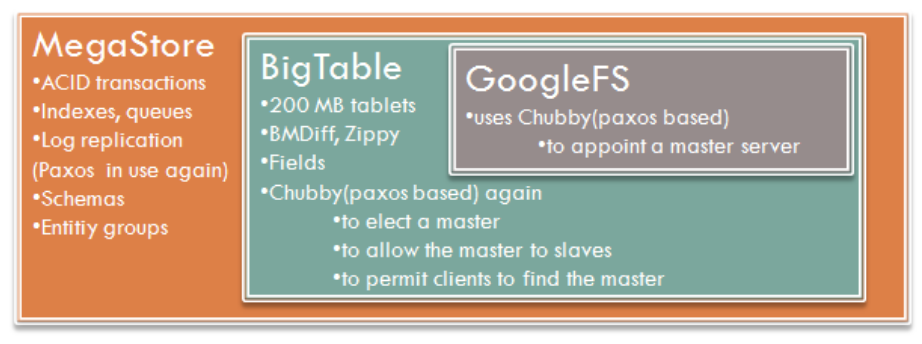
\includegraphics[width=\textwidth]{img/megastore.png}
    \end{figure}
\end{frame}
\begin{frame}
    \begin{itemize}
        \item Data divided into \textbf{entity groups} 
        \item \textbf{Replicated transaction log}  for each group
        \item Two phase commits with a paxos-based protocol 
    \end{itemize}
    \begin{figure}
        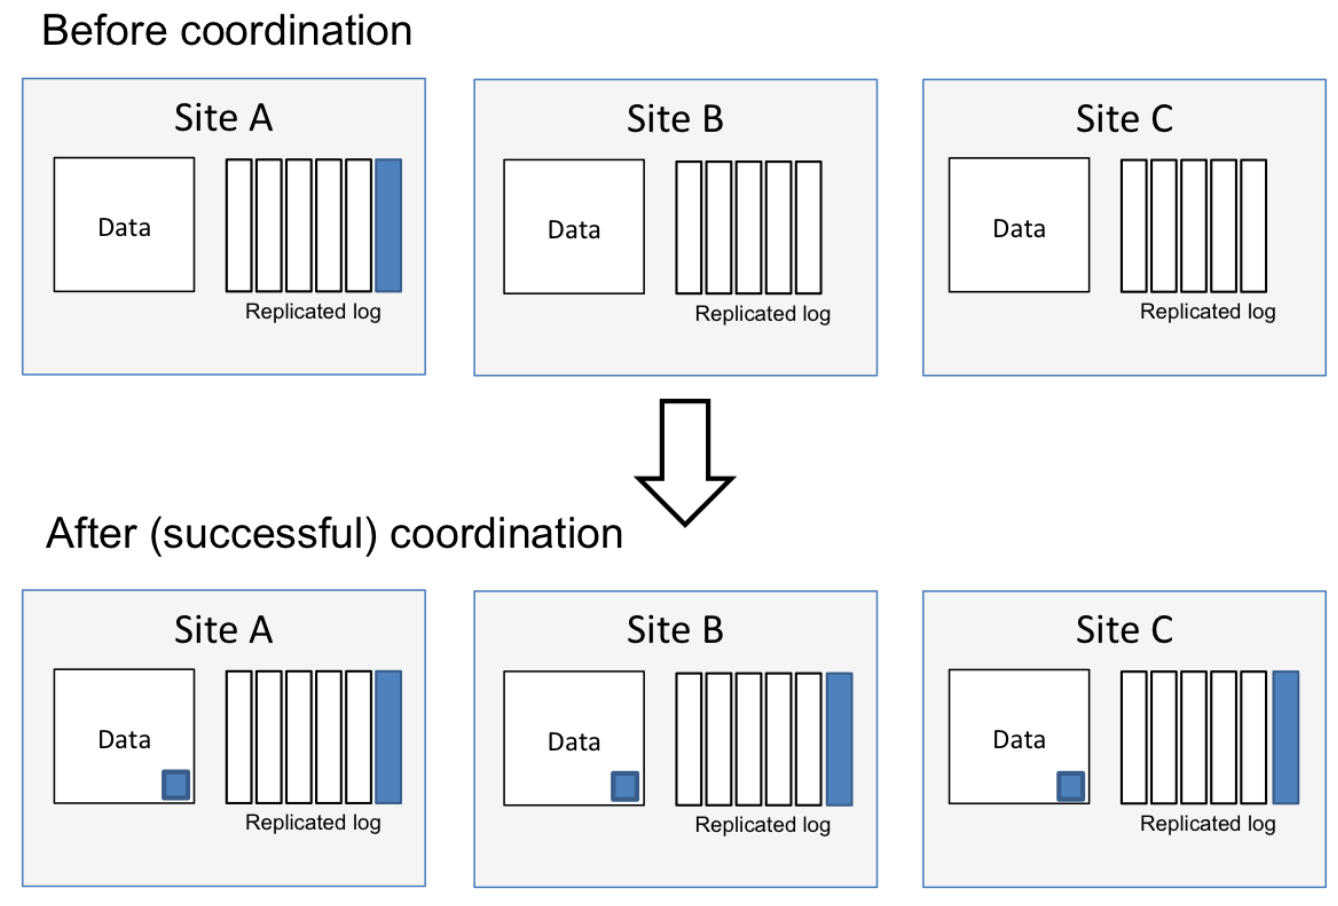
\includegraphics[scale=0.2]{img/paxos.png}
    \end{figure}
\end{frame}
\begin{frame}
    \frametitle{Issues}
    \begin{itemize}
        \item Original overview definition very informal, \textbf{really complex system}
        \item No consistency guarantee if a transaction reads multiple entity groups
    \end{itemize}
\end{frame}
\begin{frame}
    \frametitle{MegaStore CGC}

    Work by  Grov and $\ddot{\text{O}}$lveczky:
    \begin{itemize}
        \item Formalized Google MegaStore in Real-Time Maude
        \begin{itemize}
            \item 56 rewrite rules 
            \item Use  of simulation and model checking to discover bugs during development
        \end{itemize} 
        \item Introduced MegaStore CGC, an extension that provides consistency for transactions 
        accessing multiple entity groups 
    \end{itemize} 
    
\end{frame}
\begin{frame}
    \frametitle{Main ideas}

    \begin{itemize}
        \item A site participates in all updates involving the entity groups it replicates 
            \begin{itemize}
                \item Implicit ordering on these updates
                \item \textbf{Idea}: make the order \emph{explicit}
                \item Validate transactions on multiple entity groups before commit 
            \end{itemize}
            
        \bigskip
        \pause
        \item Formal test driven development 
            \begin{enumerate}
                \item Express requirements as LTL formulas
                \item Develop Real Time Maude model 
                \item Test model through simulation and model checking 
                \item Analyse failures and modify the model
            \end{enumerate}
    \end{itemize}
\end{frame}
\begin{frame}[fragile]
    \scriptsize
    \frametitle{MegaStore Maude fragments}
    \begin{lstlisting}[language=maude]
class Site | entityGroups : Configuration, localTransactions : Configuration,
            coordinator : EntGroupLogPosPairSet, egOrderings : OrderClassUpdates,
            awaitingOrder : EntGroupUpdateList .

class EntityGroup | entitiesState : EntitySet, transactionLog : LogEntryList,
                    replicas : EntityGroupReplicaSet, proposals : PaxosProposalSet,
                    pendingWrites : PendingWriteList .

class Transaction | operations : OperationList, status : TransStatus,
                    reads : EntitySet, readState : ReadStateSet,
                    writes : OperationList, paxosState : PaxosStateSet .
    \end{lstlisting}
\end{frame}
\begin{frame}[fragile]
    \scriptsize
    \begin{lstlisting}[language=maude]
crl [initiateCommit] :
    < SID' : Site |
    entityGroups EGROUPS,
    localTransactions : LOCALTRANS
    < TID : Transaction | operations : emptyOpList,
    writes : WRITEOPS, status : idle
    readState : RSTATE, paxosState : PSTATE > >
    =>
    < SID : Site |
    localTransactions : LOCALTRANS
    < TID : Transaction | paxosState : NEW-PAXOS-STATE,
    status : in-paxos > >
    ACC-LEADER-REQ-MSGS
if EIDSET := getEntityGroupIds(WRITEOPS) /\
    NEW-PAXOS-STATE := initiatePaxosState(EIDSET, TID, WRITEOPS,
    SID, RSTATE, EGROUPS)
/\ (createAcceptLeaderMessages(SID, NEW-PAXOS-STATE)) => ACC-LEADER-REQ-MSGS
    \end{lstlisting}

\end{frame}
\begin{frame}[fragile]
    \scriptsize 
    \begin{lstlisting}[language=maude]
crl [rcvAcceptAllReq] :
(msg acceptAllReq(TID, EG, (TID' LP SID OL), PROPNUM) from SENDER to THIS)
    < THIS : Site |
    entityGroups : EGROUPS
    < EG : EntityGroup | proposals : PROPSET, transactionLog : LEL > >
  =>
    < THIS : Site |
    entityGroups : EGROUPS
    < EG : EntityGroup |
    proposals : accepted(SENDER, (TID' LP SID OL), PROPNUM) ;
    removeProposal(LP, PROPSET) > >
    dly(acceptAllRsp(TID, EG, LP, PROPNUM) from THIS to SENDER), T)
if not (containsLPos(LP, LEL) or hasAcceptedForPosition(LP, PROPSET))
/\ T ; TS := possibleMessageDelay(THIS, SENDER) .       
    \end{lstlisting}
\end{frame}
\begin{frame}[fragile]
    \frametitle{LTL requirements}
    Desired Property: 
    \begin{lstlisting}[language=maude, basicstyle=\scriptsize]
    <> [] (allTransFinished /\ entityGroupsEqualOrInvalid
    /\ transLogsEqualOrInvalid /\ isSerializable)
    \end{lstlisting}

    \pause
    All replicas are equal Property:
    \begin{lstlisting}[language=maude, basicstyle=\scriptsize]
    op entityGroupsEqualOrInvalid : -> Prop [ctor] .
    
    ceq {< S1 : Site | coordinator : eglp(EG1, LP) ; EGLP,
                    entityGroups :
                    < EG1 : EntityGroup | entitiesState : ES1 > EGS1 >
        < S2 : Site | coordinator : eglp(EG1, LP) ; EGLP,
                    entityGroups :
                    < EG1 : EntityGroup | entitiesState : ES2 > EGS2 >
    REST} |= entityGroupsEqual = false if ES1 =/= ES2 .
    
    eq {SYSTEM} |= entityGroupsEqualOrInvalid = true [owise] .
    \end{lstlisting}
\end{frame}

\begin{frame}
    \huge
    Thank you for your attention!
\end{frame}
\begin{frame}[allowframebreaks]
      \nocite{*}
        \frametitle{References}
        \bibliographystyle{unsrt}
        \bibliography{bib.bib}
\end{frame}

\end{document}